\documentclass{article}

\usepackage[utf8]{inputenc}
\usepackage{setspace}
\usepackage{geometry}
\usepackage{graphicx}
\usepackage{caption}
\usepackage{indentfirst}
\usepackage{anyfontsize}
\usepackage{textcomp}
\usepackage{lipsum}
\usepackage{float}
\usepackage{changepage}
\usepackage [english]{babel}
\usepackage [autostyle, english = american]{csquotes}
\MakeOuterQuote{"}
\usepackage{amsmath}

\graphicspath{}



\title{Bifurcation in Fishing Models with Holling's Type II Term}
\author{Geneva Porter}
\date{05 November 2018}

%\begin{figure}[H]
%\centering{\includegraphics[width=10cm]{FILENAME.eps}}
%	\caption{CAPTION}
%\end{figure}

%$\begin{bmatrix}
%11      & 12  \\
%21      & 22  \\
%\end{bmatrix}$

\begin{document}
	
\begin{titlepage}
\maketitle
\thispagestyle{empty}


\begin{center}
	
\large \it San Diego State University 
	
Professor J Mahaffy, Math 636

\end{center}
\end{titlepage}

\subsection*{Model Description}
The following equation is a simple population model for harvesting fish:

\begin{center}
	$\dfrac{dF}{dt}=0.2F(1-\dfrac{F}{100})-\dfrac{hF}{1+0.02F}$
\end{center}

\subsubsection*{Malthusian, Logistic, and Holling's Terms}
 Each term in this differential equation equates to a behavior describing population dynamics. The model itself describes the rate of change in some population of fish, with consideration towards harvesting practices. The first term, 0.2F, is the exponential Malthusian growth term and specifies the reproduction rate of the fish without limitations and with abundant resources. The second term, $1-F/100$, represents the logistic growth factor that slows growth due to limited resources. This term also indicates that the carrying capacity is 100 when we are only considering logistic growth. If the population were to exceed this number, we would see population decline. The last term is the Holling's type II term. It signifies the rate of harvesting as influenced by the density of the fish population. Harvesting increases as population increases, but then levels off once the population reaches the carrying capacity. This is similar to a predator-prey model, which would signify the predator (fishermen) being satiated by the prey (fish). If we take the limit of this term, we can see that as $F$ gets large, the term approaches $50h$, which would signify the rate of population decline due to harvesting. Graphing this model would show us the equilibria ($x$-intercepts) and maximum growth rate (critical point). 

\subsubsection*{Constant Harvesting Term}
If we eliminated Holling's Type II term and only use $h$ for our third term, then we would have a population model with constant harvesting. Notice that this would be structurally identical to the logistic model, but shifted downward on the $y$-axis. This model would also indicate that there is a threshold where the population must be in order to increase toward equilibrium. This means that when there is a negative value for $dF/dt$ at a small population, constant harvesting will push the population to extinction. 

\subsubsection*{Proportional Fishing}
Another alternative to the Holling's Type II term is a proportional harvesting term. These are similar in that the decline in population results in a decline in harvesting, much like with net fishing--only a proportion of the population is captured. Also like the Holling's Type II term, we will always have an equilibrium at 0. However, using this term would also imply that harvesting would be very large for large populations of fish, which may not be entirely realistic.

\pagebreak

\subsection*{Zero Harvesting}
If we take our harvesting term to be zero, we are left with a simple logistic model:

	\begin{center}
		$\dfrac{dF}{dt}=0.2F(1-\dfrac{F}{100}) $
	\end{center}
	
Setting $dF/dt=0$ gives us two equilibria at $F=0$ and $F=100$, the carrying capacity. As usual, this population model has an unstable equilibria at the extinction point and a stable equilibria at the carrying capacity. We can show this by taking the derivative of this equation and evaluating it at the equilibria to determine stability:

\begin{center}
	For $h=0$, $\dfrac{d^2F}{dt^2}=0.2-.004F=$
$\begin{cases} $
$0.2 \hspace{5mm}$ when $F=0 \\$
$-0.2 \hspace{2mm}$ when $F=100$
$\end{cases}$
\end{center}

This confirms our earlier statement on the stability of the model. The fish population tends to grow rapidly when very small, until the growth rate slows to zero and an equilibrium is achieved at the carrying capacity. The phase portrait indicates that the population will grow to 100 when starting above zero, and will decrease to 100 if it is larger. Below is a graph of the model and its one-dimensional phase portrait.


\begin{figure}[H]
\centering{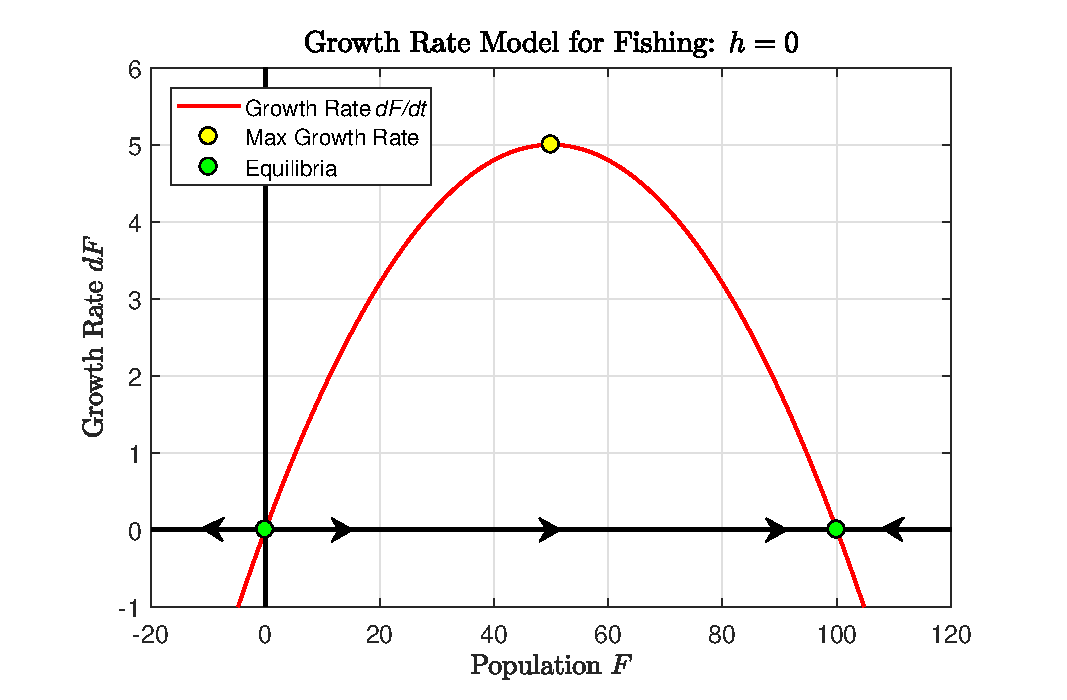
\includegraphics[width=12cm]{f1.eps}}
	\caption*{\hspace{3mm} \textbf{Figure 1}}
\end{figure}

\pagebreak

\subsection*{Harvesting with $0\leq h\leq0.25$}

If we allow the harvesting term to increase, we find that the dynamics of the model change. While we will maintain our equilibrium at $F=0$, our carrying capacity and maximum growth rate will decrease. In order to calculate where these changes will occur with respect to $h$, we must find the bifurcation points. To to this, we first find our equilibrium points, as a function of $h$:

\begin{center}
	$\dfrac{dF}{dt} = 0 \hspace{5mm} \longrightarrow \hspace{5mm} F_e = $
	$\begin{cases}
	0 \\
	25-25\sqrt{9-40h} \\
	25+25\sqrt{9-40h} \\
	\end{cases}$
\end{center}

Note that real equilibrium values require $h\leq0.225$. Next, we find the derivative of $dF/dt$ (we'll call this equation $g$ for simplicity). We can then plug in our equilibrium points for the values of $F$ into $g$, and set $g$ equal to zero.

\begin{center}
	$g(F,h) = \dfrac{d^2F}{dt^2} = \dfrac{0.2-h+(4\cdot10^{-3})F-(8\cdot 10^{-5})F^2-(1.6\cdot 10^{-6})F^3}{(1+0.02F)^2}$
\end{center}


\begin{flushleft}
\hspace{20mm}		$g(F_e,h)=\begin{cases}
1/5-h \vspace{3mm}\\
\dfrac{(-1.8+8h)-(0.6-2h)(\sqrt{9-40h})}{9-20h+3\sqrt{9-40h}} \vspace{3mm} \\
\dfrac{(-1.8+8h)+(0.6-2h)(\sqrt{9-40h})}{9-20h+3\sqrt{9-40h}} \\
\end{cases}$

\end{flushleft}

Setting each of these evaluations to zero and solving for $h$ gives us a transcritical bifurcation point at $h_1=0.2$ and a saddle node bifurcation point at $h_2=0.225$. Figure 2 shows a diagram of these bifurcations, which will be discussed further in below. Next, we will discuss how this model behaves around these bifurcation points and how they are classified.

\begin{figure}[H]
	\centering{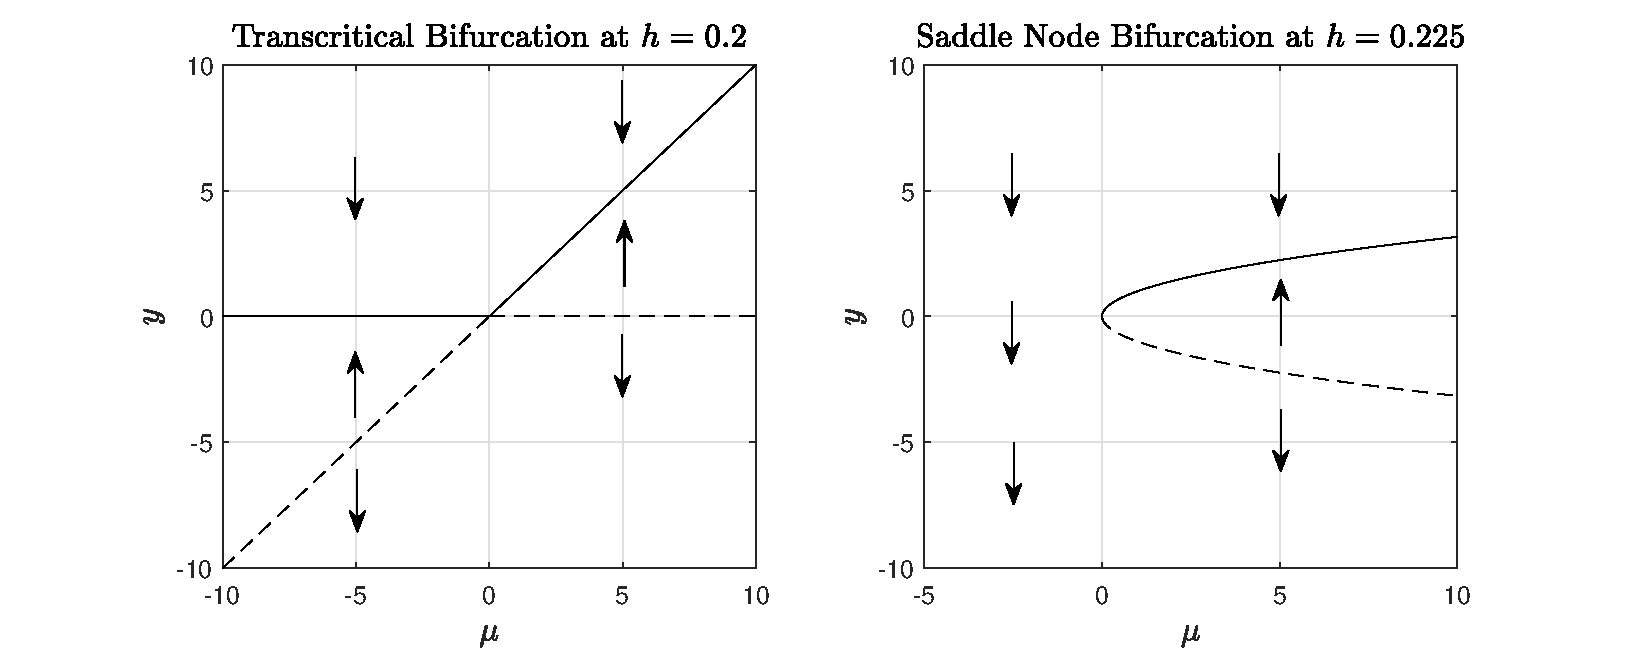
\includegraphics[width=15cm]{f2.eps}}
	\caption*{\textbf{Figure 2}}
\end{figure}

\pagebreak

\subsubsection*{Discussion for $h=0.2$}
We will examine the bifurcation at $h=0.2$ first. We can classify this bifurcation by examining what happens when $h$ is marginally larger or smaller than 0.2. We will choose $\delta=0.01$ as the as the increment for which we will disturb the value of $h$. The simplest way to investigate this is to examine the graph of $dF/dt$ vs. $F$ for these values of $h$. Figure 3 shows this comparison, along with the phase behavior on the $F$-axis. Solid circles indicate stable points, while hollow circles indicate unstable points. Some equilibrium points are extended on a vertical line for a clearer phase portrait view.

\begin{figure}[H]
	\centerline{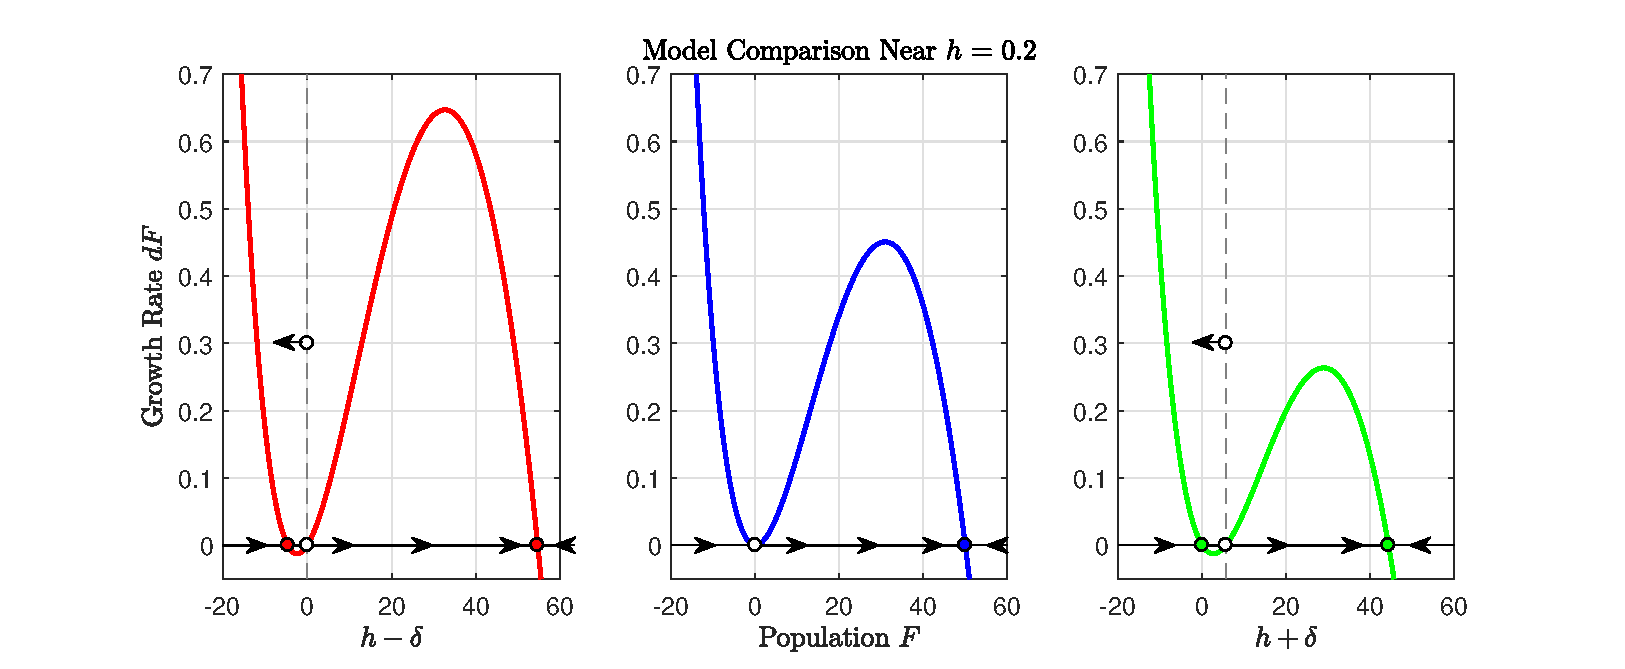
\includegraphics[width=18cm]{f3.eps}}
	\caption*{\textbf{Figure 3}}
\end{figure}

		$h-\delta: \begin{cases}$
$e_{1_{-\delta}} = -4.580$, stable$\\$
$e_{2_{-\delta}} =  0$, unstable $\\$
$e_{3_{-\delta}} = 54.508$, stable $\\$
$\end{cases}$\hspace{5mm}
$h: \begin{cases}$
$e_{1} = 0$, unstable$\\$
$e_{2} =  50$, stable $\\$
$\end{cases}$\hspace{5mm}
$h+\delta: \begin{cases}$
$e_{1_{+\delta}} = 0$, stable$\\$
$e_{2_{+\delta}} =  5.635$, unstable $\\$
$e_{3_{+\delta}} = 44.365$, stable $\\$
$\end{cases}$

\vspace{5mm}

As we increase the parameter $h$ from $h-\delta=0.19$ to $h+\delta=0.21$, we can see that the number of fixed points goes form 3 to 2 and back to 3 again. We can also see that zero is always a fixed point, and it changes stability at the bifurcation point. Zero is unstable when $h\leq0.2$ and stable when $h>0.2$. This indicates that $h=0.2$ is a transcritical bifurcation point. If we examine this model where $h=0.2$, we can see that it behaves much like a logistic model for $F\geq0$. The extinction equilibrium is unstable, and the population will tend toward a carrying capacity of 50. If we reduce the harvesting parameter by a small amount, we still see behavior similar to the logistic equation. There is an unstable equilibrium at 0, and the population will tend toward a carrying capacity of $\approx55$. There is a third equilibrium on the negative $F$ axis, but since that correlates to a negative population, its dynamics are not realistic. For the harvesting parameter values at or below 0.2, the population grows rapidly from low numbers, reaches a maximum growth rate, and the growth rate slows to zero at the carrying capacity. Perturbations away from the carrying capacity equilibrium will not effect population dynamics long-term, as the population will tend to stay around that number. When we increase the harvesting factor by a small amount, the population dynamics begin to change more aggressively, and the model gives rise to an extinction threshold. The threshold equilibrium at $\approx6$ is unstable, meaning that a population below this number will die out, while a population above this number will grow toward a carrying capacity of $\approx44$. 

\subsubsection*{Discussion for $h=0.225$}

For a harvesting parameter around $h=0.225$, we see a significant tipping point. Figure 4 shows our model with small perturbations of $h$ of $\delta=0.01$. 

\begin{figure}[H]
	\centerline{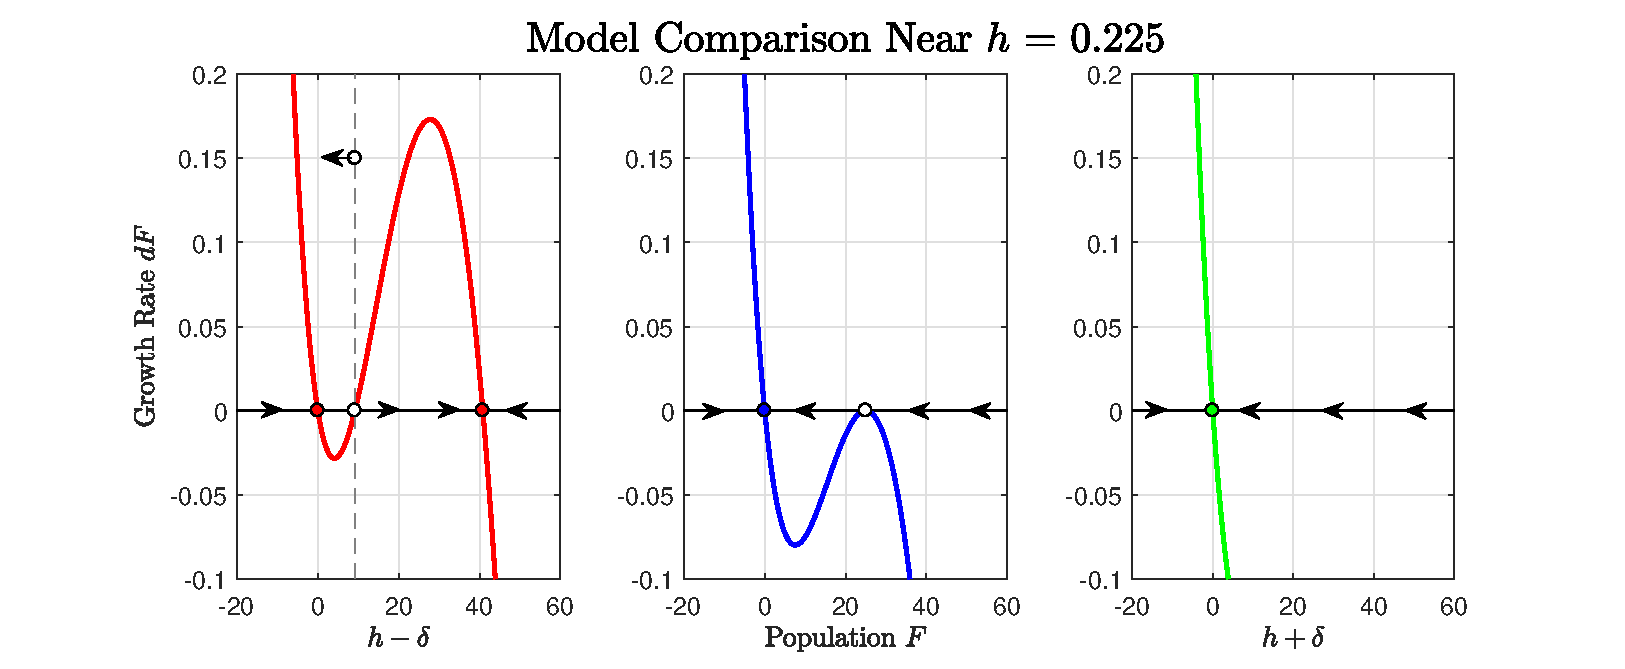
\includegraphics[width=18cm]{f4.eps}}
	\caption*{\textbf{Figure 4}}
\end{figure}

\begin{flushleft}
	$h-\delta: \begin{cases}$
$e_{1_{-\delta}} = 0$, stable$\\$
$e_{2_{-\delta}} =  9.189$, unstable $\\$
$e_{3_{-\delta}} = 40.811 $, stable $\\$
$\end{cases}$\hspace{5mm}
$h: \begin{cases}$
$e_{1} = 0$, stable$\\$
$e_{2} =  25$, unstable $\\$
$\end{cases}$\hspace{5mm}
$h+\delta: \begin{cases}$
$e_{1_{+\delta}} = 0$, stable$\\$
$\end{cases}$

\end{flushleft}

\vspace{5mm}

We can see here that our model goes from 3 fixed points to 2 to 1. This "disappearance" of two fixed points indicates that they "collided" with one another and were then eliminated. This type of bifurcation is classified as a saddle node or "blue skies" bifurcation. Here we can see some dramatic dynamical changes. If a harvesting factor of $0.225$ is enforced, the fish will quickly die out to extinction. The extinction equilibria is the only stable one, indicating that any population between 0 and 25 will die. We can't say that a carrying capacity exists in this sense either, as the growth rate is negative for all populations. An equilibrium at 25 suggests that a population could theoretically exist if it never deviated from that equilibrium, but of course that is not realistic. Any populations above 25 will also decline to extinction. Setting $h$ just a bit smaller at least allows for some population growth and a carrying capacity. The threshold that appeared for $h>0.2$ is now at $\approx9$, so as long as the population stays above that number then they will eventually reach a carrying capacity of $\approx41$. A population less than nine would of course be harvested to extinction. Now we can look at a small increase from $h=0.225$. Here there is only one equilibrium point at zero, it is unstable, and the growth rate for all populations is negative. The steepness of the curve suggests that the population will decline very rapidly for any positive population. We can conclude that this model predicts that a harvesting level at or above 0.225 will drive the fish to extinction.




\end{document}





































